\hypersetup{linkcolor=blue}
\chapter{Does Path length impact Latency for Netflix?} \label{chapter:7}
In this chapter we will analyse the content delivery on the Internet, we will analyse the traceroute measurements that we have in the dataset. 
The traces are towards Netflix OCA servers and towards ISPs content caches which hold the Netflix audio and video content. As mentioned in \cite{vietpam2018}, 
We used scamper \cite{scamper} on around 100 dual-stacked SamKnows probes \cite{samknows}. The test runs \textit{paris-traceroute} \cite{paris} for IPv4 and IPv6 
every hour, towards Netflix OCA servers. The attribute that we are going to analyse is \textit{TTL (Time-To-Live)} \cite{rfc3443} between the client and the Netflix OCA server. 
Other attributes that we will analyse here are the \textit{TCP Connect Times and the Pre-buffering Durations}, and we will see the impact of path lengths (TTL) over these 
latency attributes. 

\section{Temporal Analysis}

\begin{figure}[!ht]
	\centering
	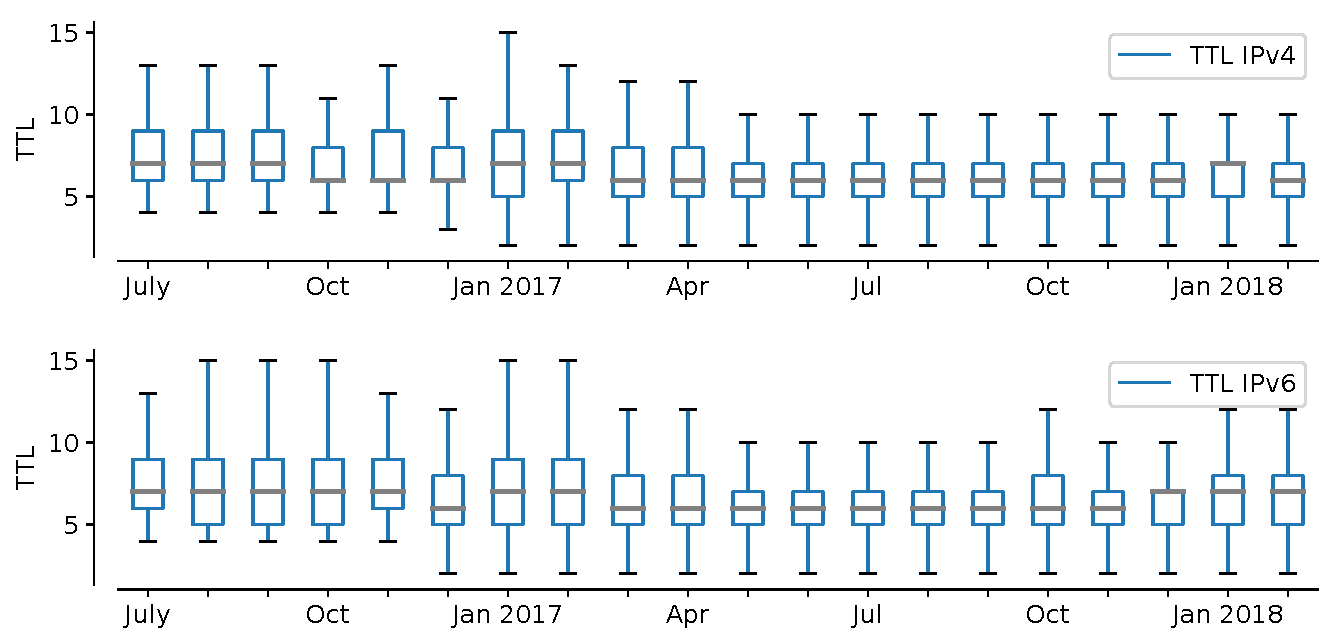
\includegraphics[keepaspectratio, height=5cm, width=15cm]{figures/traceroute/netflix-traceroute-rtt-ttl-separate-new.pdf}
	\caption[TTL Boxplot Absolute]{Boxplot of TTL absolute values over IPv4 and IPv6, by months and across all the probes. For both the address family's, no significant changes could be observed, and the median along every month is around 5-8 over IPv4 and IPv6.}
	\label{fig:TTL Boxplot Absolute}
\end{figure}

We wanted to see the path lengths changes over the entire duration of the dataset and the impact on the latency. 
We are looking at the maximum TTL values i.e. the number of hops traversed to reach the destination host (Netflix OCA here). 
Also, we are considering the TCP Connect Times and Pre-Buffering Duration along this timeline, to see the impact on the latency with respect to path length. 
As the \textit{scamper} test ran every hour for both IPv4 and IPv6, therefore, the traceroute measurements can be compared for both the address family's. 
We already computed the difference between the two address family's, refer table \textit{deltas} in \cref{table:deltas}. 
As Viet \cite{viet} did in his study, we are using the "COMPLETED" measurements here and are considering the maximum TTL values here for computing the deltas, 
reason for using maximum TTL value is that most of the clients would prefer faster connection time irrespective of the path length and the intermediate hops 
between the source and the destination hosts. 

\begin{figure}[!ht]
	\centering
	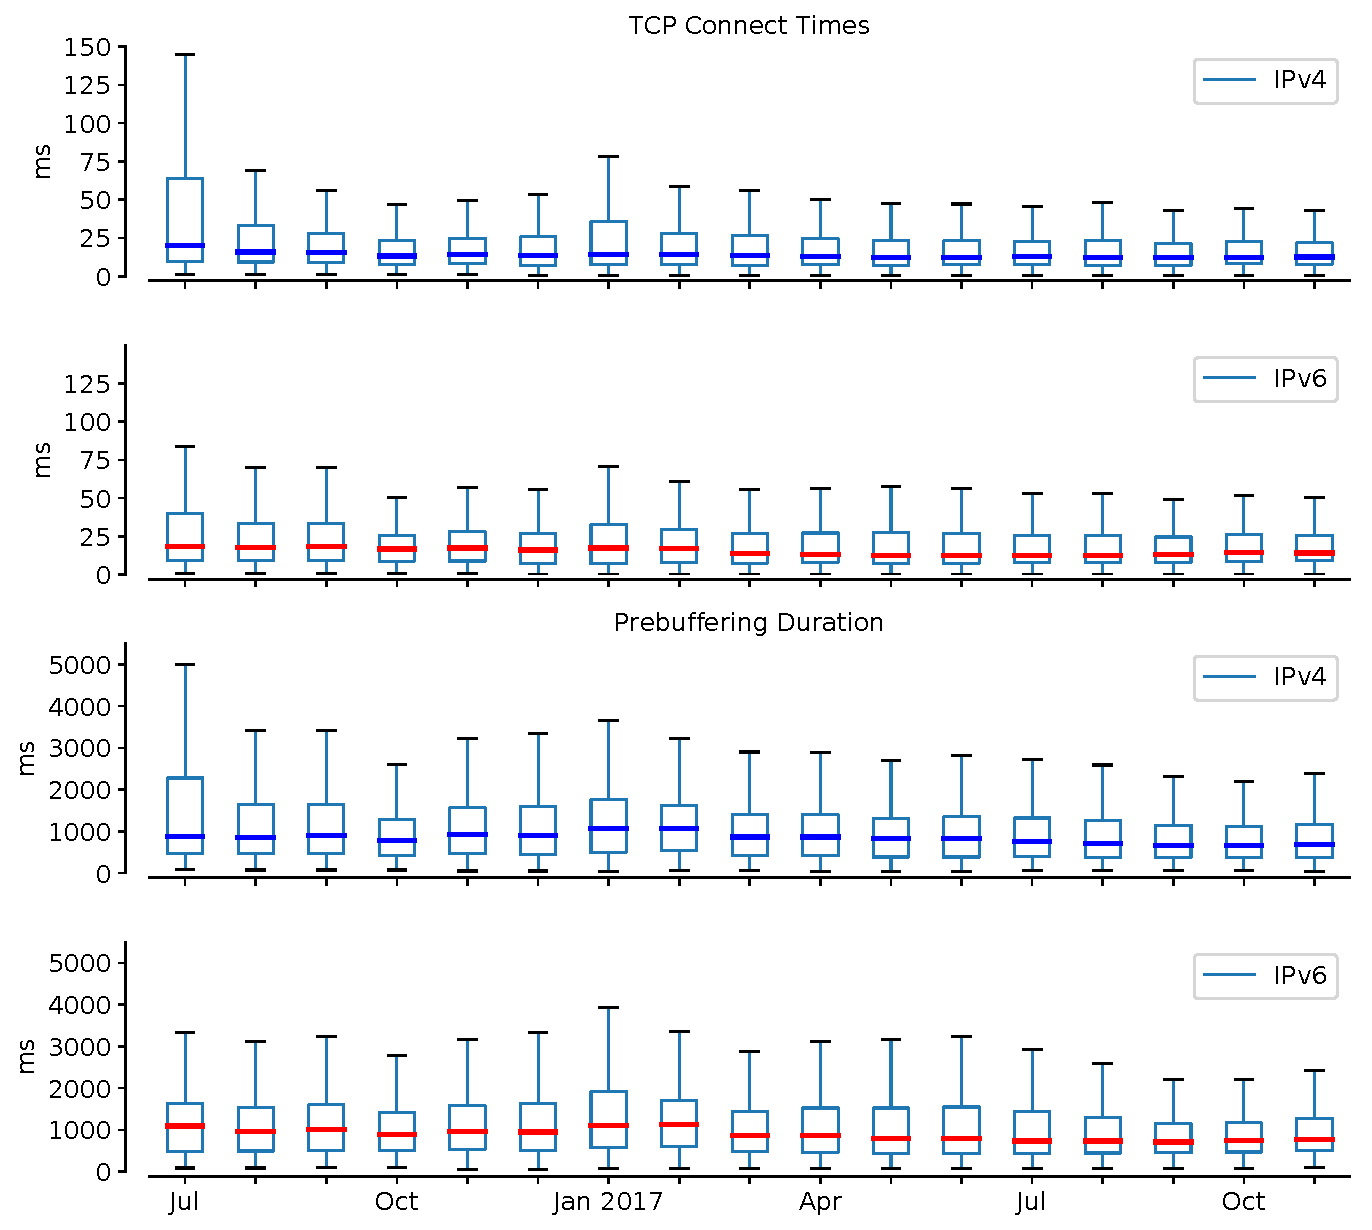
\includegraphics[keepaspectratio, height=8cm, width=15cm]{figures/traceroute/netflix-delay-boxplot-separate.pdf}
	\caption[TCP Connect Times and PreBuffering Duration Boxplot Absolute]{Boxplot of TCP connect times and Pre-buffering duration over the entire duration, across all probes. We see a similar pattern over both IPv4 and IPv6 address family's.}
	\label{fig:TCP Connect Times and PreBuffering Duration Boxplot Absolute}
\end{figure}

We will first consider the absolute values for the attributes over IPv4 and IPv6. As can be seen in \cref{fig:TTL Boxplot Absolute} the first and third quartiles for 
maximum TTL values over IPv4 and IPv6 lies between 0-15 hops for the entire duration, and the median is between 5-8 hops for individual months. Also, we see a steady graph i.e. 
no significant changes during the entire duration. Similarly, we can see the absolute values over IPv4 and IPv6 for the TCP Connect Times and Pre-buffering Durations 
for the whole timeline, in \cref{fig:TCP Connect Times and PreBuffering Duration Boxplot Absolute}. Here, we have converted the TCP connect times and Pre-buffering duration 
to 'ms' to get a better understanding. As can be seen, there are no major changes along the whole time-line and, we cannot see much difference between IPv4 and IPv6 performance, 
so it would be good to compare the deltas here. 

\FloatBarrier

\begin{figure}[!ht]
	\centering
	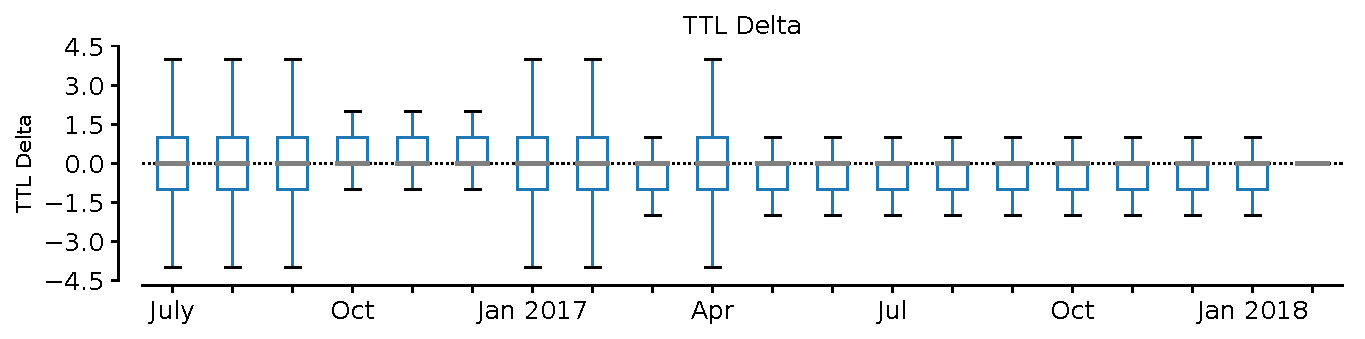
\includegraphics[keepaspectratio, height=5cm, width=10cm]{figures/traceroute/netflix-traceroute-rtt-ttl-deltas-new.pdf}
	\caption[TTL Boxplot Delta]{Boxplot of TTL delta, along the entire duration and across all probes. No significant changes can be seen here, and the median stays around 0 indicating IPv6 performs at par with IPv4. }
	\label{fig:TTL Boxplot Delta}
\end{figure}

\begin{figure}[!ht]
	\centering
	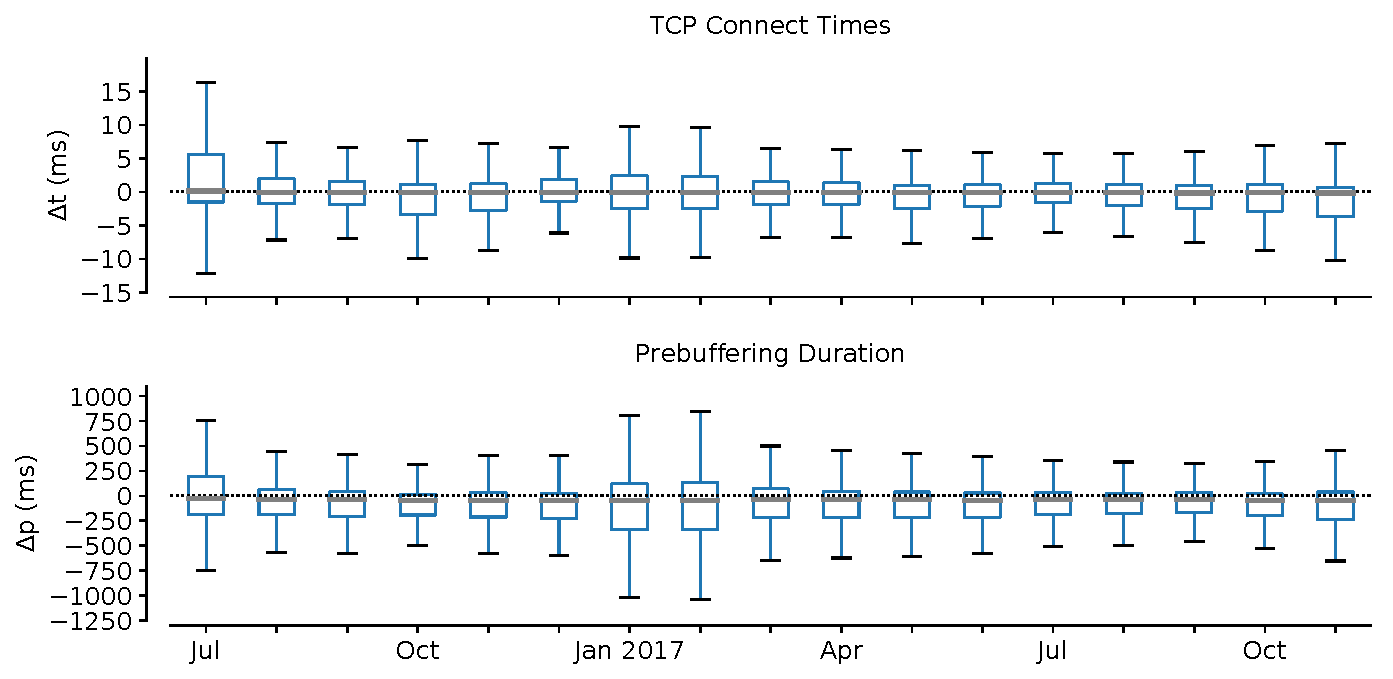
\includegraphics[keepaspectratio, height=5cm, width=15cm]{figures/traceroute/netflix-delay-boxplot.pdf}
	\caption[TCP and Prebuffering Duration Boxplot Delta]{Boxplots of TCP connect times and Pre-buffering duration deltas, across all probes. The median remains around 0 indicating IPv6 performance is comparable to IPv4.}
	\label{fig:TCP and Prebuffering Duration Boxplot Delta}
\end{figure}

As \textit{deltas} here are computed as the difference between IPv4 and IPv6, the positive values indicate that the IPv6 need less hops to reach the destination. 
Ideally, as IPv6 adoption has increased, with increased deployment of IPv6 infrastructure and support, the deltas should be around 0, indicating that IPv6 is on par with IPv4. 
We plotted the deltas as a Bocplot, and as we can see from \cref{fig:TTL Boxplot Delta}, there are no significant changes that could be seen along the entire duration. 
The median is along 0, which indicates that the IPv6 performed at par with IPv4 in terms of TTL. The reason for varying first and third quartile among certain months is unclear.  
Similarly, for TCP connect times and Pre-buffering duration, the median stays steady around 0, indicating similar performance over IPv4 and IPv6. 

The above analysis provide a holistic view of the traceroute measurements towards Netflix OCA servers, because the SamKnows probes are located all over the world. 
Also, it can be seen that no drastic changes could be seen over the last two years. 

\FloatBarrier

\section{Path Length and Latency Comparison} 

Here, we are considering the path length across all probes for the entire duration without considering the time factor. \cref{fig:TTL CDF Absolute} describes the CDF of median TTL over the entire duration. Here, around 93\% of the IPv4 paths have a TTL of 13 or lower, while 93\% of the paths over IPv6 have a TTL of 12 or lower. As the number of paths are similar over both address family's. the data indicates that more paths are shorter over IPv6 as compared to IPv4. This can also be seen from the figure, as IPv6 datapoints (Red) are above the IPv4 datapoints (Blue) on the graph. The difference is not that prominent and thus, both the address family's showing comporable performance. 

\begin{figure}[!ht]
	\centering
	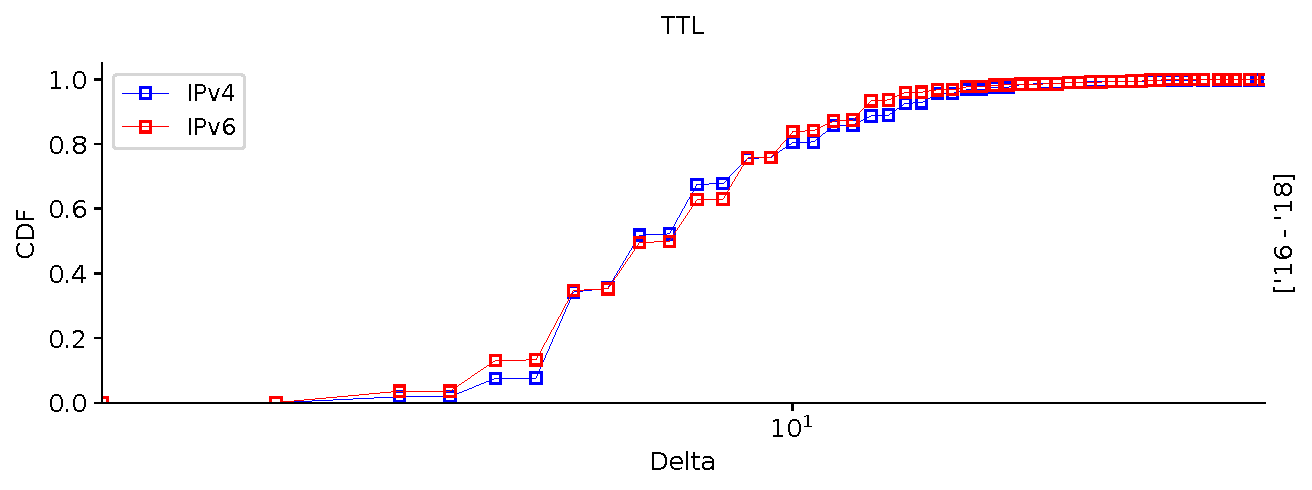
\includegraphics[keepaspectratio, height=5cm, width=15cm]{figures/traceroute/netflix-traceroute-median-ttl-cdf-separate.pdf}
	\caption[TTL CDF Absolute]{CDF of TTL over IPv4 and IPv6. Both the curves, IPv4 and IPv6, are largely overlapping indicating similar performance over both the address family's.}
	\label{fig:TTL CDF Absolute}
\end{figure}

\FloatBarrier

For TCP Connect times and Pre-Buffering duration, we have already discussed the \cref{fig:Connect Time and Prebuffering Duration CDF Absolute} in \hyperref{section:tcppd}, 
we cannot see much difference in the performance over IPv4 and IPv6 and therefore, both the address family's show similar latency. 

We now can conclude that path lengths over IPv6 and IPv4 are comparable and the latency i.e. TCP connect times and Pre-Buffering duration are also comparable over 
both the address families. We therefore need to see the deltas for better comparison.

\begin{figure}
	\centering
	\begin{minipage}{0.5\textwidth}
		\centering
		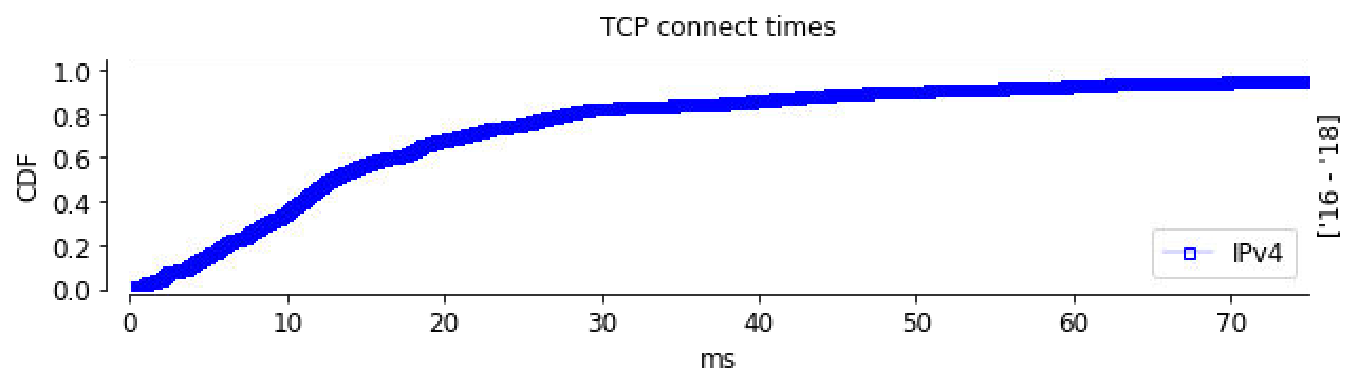
\includegraphics[keepaspectratio, height=5cm, width=8.5cm]{figures/tcp/netflix-syn-time-absolute-difference-v4.pdf}
	\end{minipage}
	\begin{minipage}{0.5\textwidth}
		\centering
		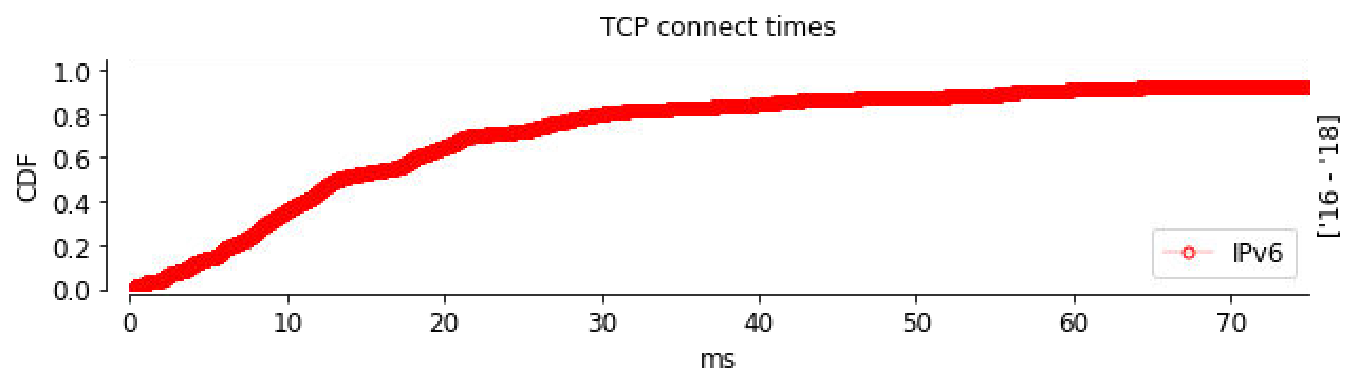
\includegraphics[keepaspectratio, height=5cm, width=8.5cm]{figures/tcp/netflix-syn-time-absolute-difference-v6.pdf}
	\end{minipage}
	\begin{minipage}{0.5\textwidth}
		\centering
		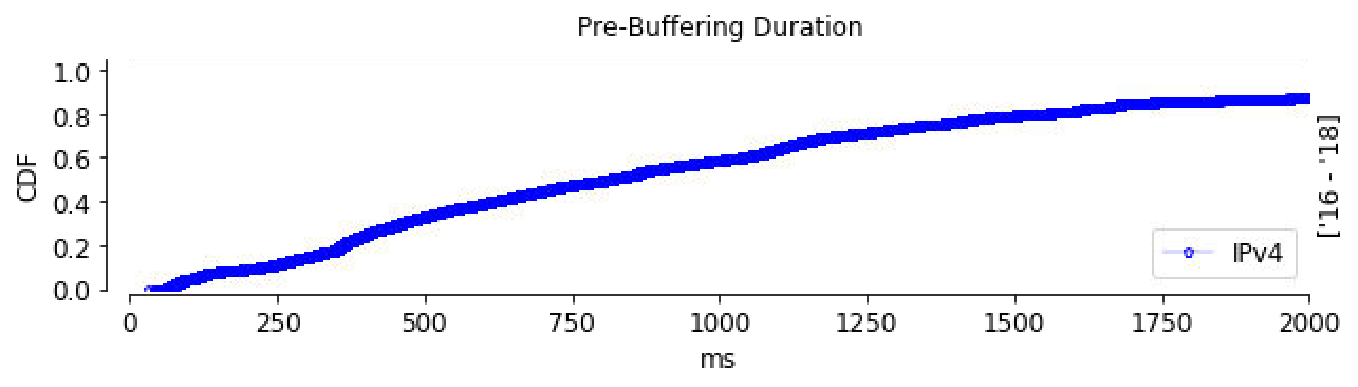
\includegraphics[keepaspectratio, height=5cm, width=8.5cm]{figures/tcp/netflix-prebuffering-duration-absolute-difference-v4.pdf}
	\end{minipage}
	\begin{minipage}{0.5\textwidth}
		\centering
		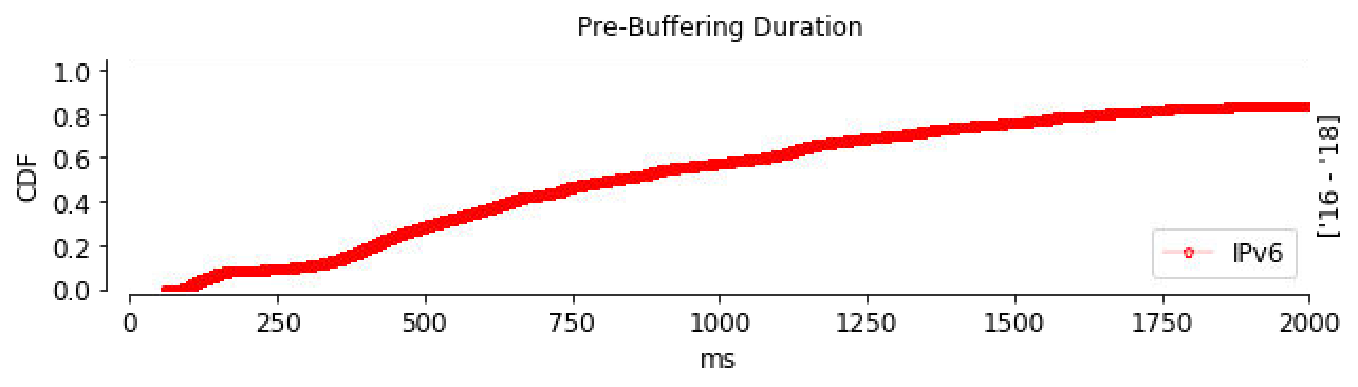
\includegraphics[keepaspectratio, height=5cm, width=8.5cm]{figures/tcp/netflix-prebuffering-duration-absolute-difference-v6.pdf}
	\end{minipage}
	\caption[Connect Time and Prebuffering Duration CDF Absolute]{CDF of TCP Connect Times and Prebuffering Duration for IPv4 and IPv6. We cannot see much difference between the address family's.}
	\label{fig:Connect Time and Prebuffering Duration CDF Absolute}
\end{figure}

\FloatBarrier

\section{Path Latency and Latency Deltas}

To get a more clear picture, we plotted the distribution of TTL, TCP connect times, and Pre-buffering duration. We can see the TTL and TCP connect times deltas in \cref{fig:TTL and TCP CDF Delta}. 
The plot shows that around 31\% of the pairs had a median TTL of less than 0, whereas around 33\% of the pairs had a positive delta which indicates less number of hops over IPv6. 
The remaining 36\% of the median TTL deltas are located at 0, which illustrates that fraction of median TTL over IPv6 being shorter, equal or faster to IPv4 are somewhat same. 
If we compare the TCP connect times, then the distribution shows that 57\% of the connections are slower over IPv6, with 13\% of them at least 10 ms slower.
Also, if we check the Pre-Buffering duration deltas in \cref{fig:TTL and PreBuffering Duration CDF Delta}, we can see from the distribution that around 70\% of the connections 
are slower over IPv6.

\begin{figure}[!ht]
	\centering
	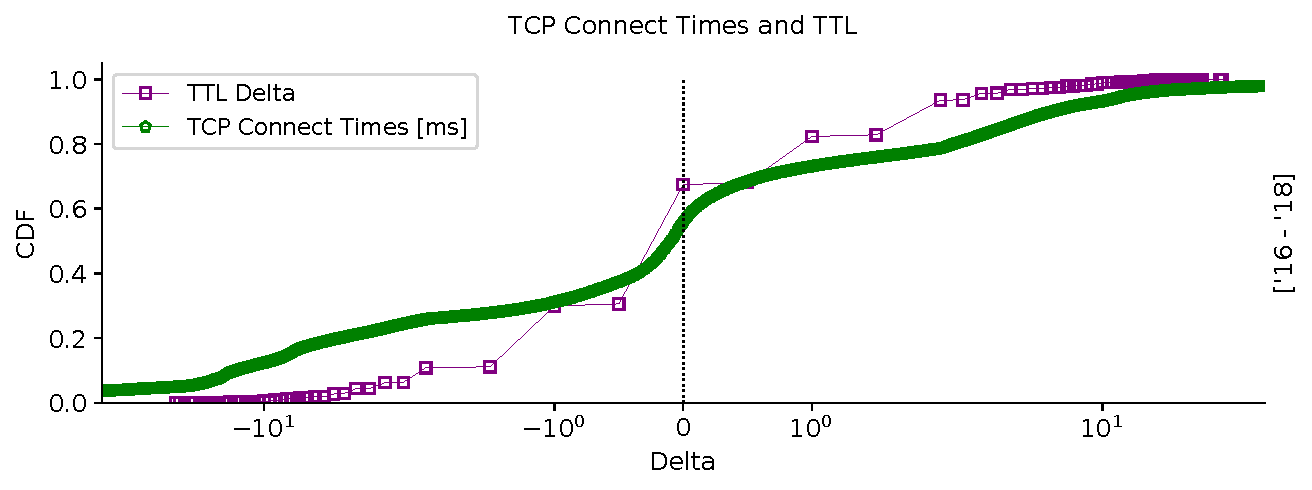
\includegraphics[keepaspectratio, height=5cm, width=15cm]{figures/traceroute/netflix-traceroute-median-ttl-tcp-cdf.pdf}
	\caption[TTL and TCP CDF Delta]{CDF of TCP Connect Times and TTL over the entire duration and across all probes. Here, TTL over IPv4 is shorter, equal or longer in about one/third of the measurements compared to IPv6. Regarding TCP Connect times, the distribution here shows that 57\% of the connections are slower over IPv6, with 13\% of them at least 10 ms slower.}
	\label{fig:TTL and TCP CDF Delta}
\end{figure}

\begin{figure}[!ht]
	\centering
	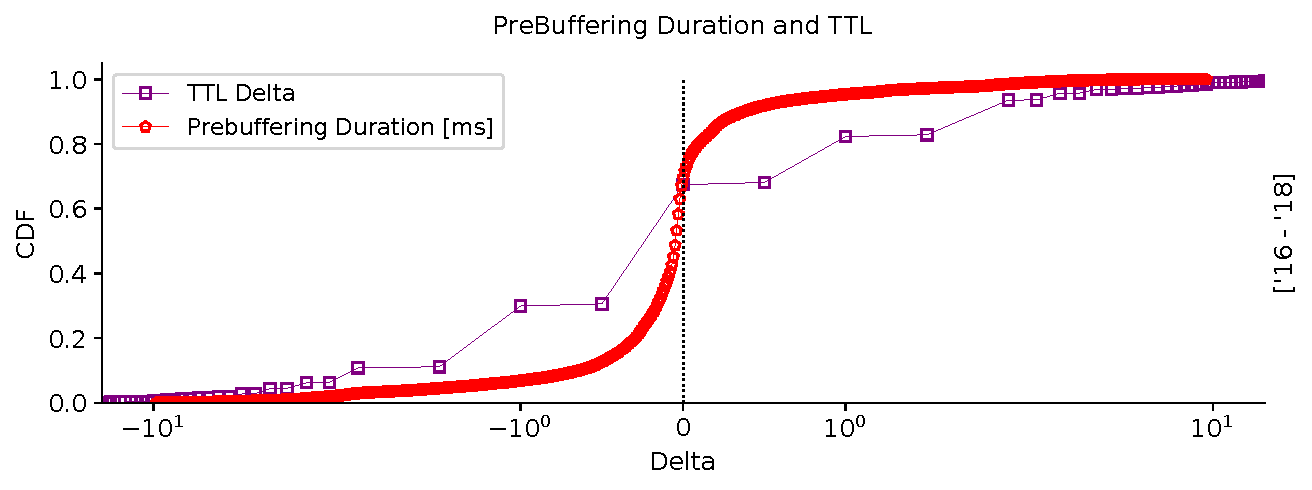
\includegraphics[keepaspectratio, height=5cm, width=15cm]{figures/traceroute/netflix-traceroute-median-ttl-pd-cdf.pdf}
	\caption[TTL and PreBuffering Duration CDF Delta]{CDF of TTL and Pre-buffering Duration over the entire duration and across all probes.Here, TTL over IPv4 is shorter, equal or longer in about one/third of the measurements compared to IPv6. Regarding the Pre-Buffering Duration, distribution shows that around 70\% of the connections are slower over IPv6.}
	\label{fig:TTL and PreBuffering Duration CDF Delta}
\end{figure}

Going forward, we will analyse the destinations based on CAIDA's \cite{caida} classifications, identifying the content caches and the OCA hosts.

\FloatBarrier

\section{Content Caches}

Content Caches helps reduce the access time to frequently accessed data, as they mirror the content temporarily so as to reduce the load on the original hosts. 
It is expected and believed that the TTL and Latency should be lower incase a cache is hit as when the origin server (Netflix OCA here) is hit. 
The reason for this is that the caches are situated closer to the client which make the requests, generally at the ISP networks (refer \hyperref{chapter:Related Work}).
 We can identify the the content caches by comparing the AS Number of the source IP (\cref{table:source} with the AS Number of the destination IP (\cref{table:destination}). 
 If there is a match then it is a cache located near to the probe and the client request never left the ISP network.

Viet in \cite{viet} mentioned four different scenarios to identify a cache. These are,

\begin{enumerate}
  \item IPv4 only cache, i.e. no cache for IPv6.
  \item IPv6 only cache, i.e. no cache for IPv4.
  \item Both Caches, i.e. ISP caches identified for both IPv4 and IPv6.
  \item No ISP cache hit for niether IPv4 or IPv6.
\end{enumerate}

The above four scenarios could be visualized if we split up the graphs in \cref{fig:TTL and TCP CDF Delta} and \cref{fig:TTL and PreBuffering Duration CDF Delta}, 
based on the above four conditions. Considering only the TTL, hypothetically, an IPv4 only cache should be on the negative side of the x-axis as the paths will be 
shorter for IPv4 cache. Similarly, for IPv6 only cache, the shift should be on the positive side of the x-axis. For both the caches, the values should be around 0. 
If this isn't the case then the possible reason can be regarding the network infrastructure and configuration of the ISP caches. For case 4, where there isn't any cache, 
the plot should be a less steep curve.

\begin{figure}[!ht]
	\centering
	\begin{minipage}{0.5\textwidth}
		\centering
		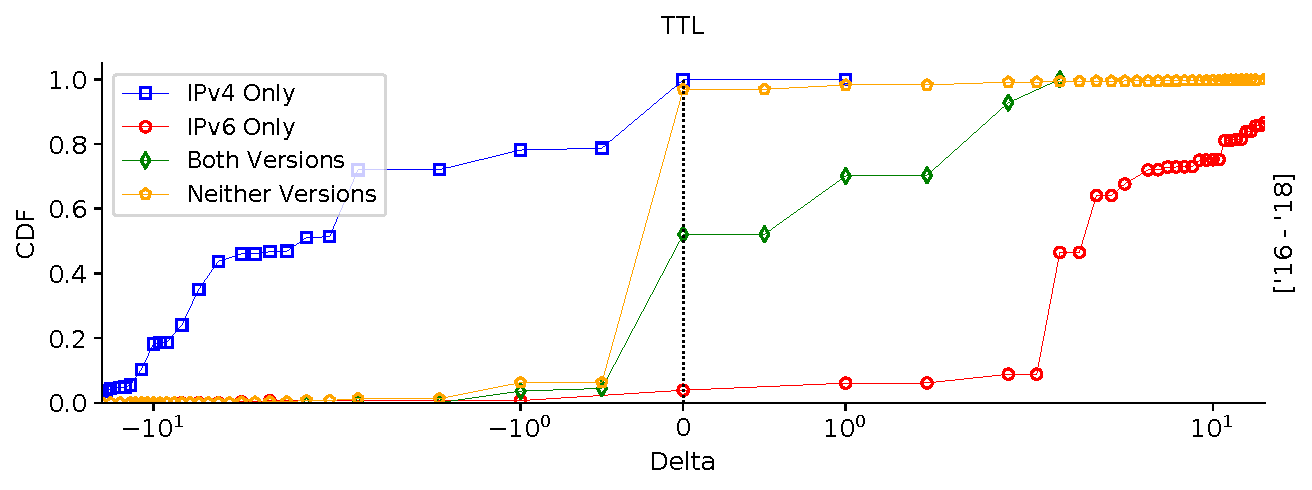
\includegraphics[keepaspectratio, height=5cm, width=8.5cm]{figures/traceroute/netflix-traceroute-median-ttl-cache-pair-cdf.pdf}
	\end{minipage}
	\begin{minipage}{0.5\textwidth}
		\centering
		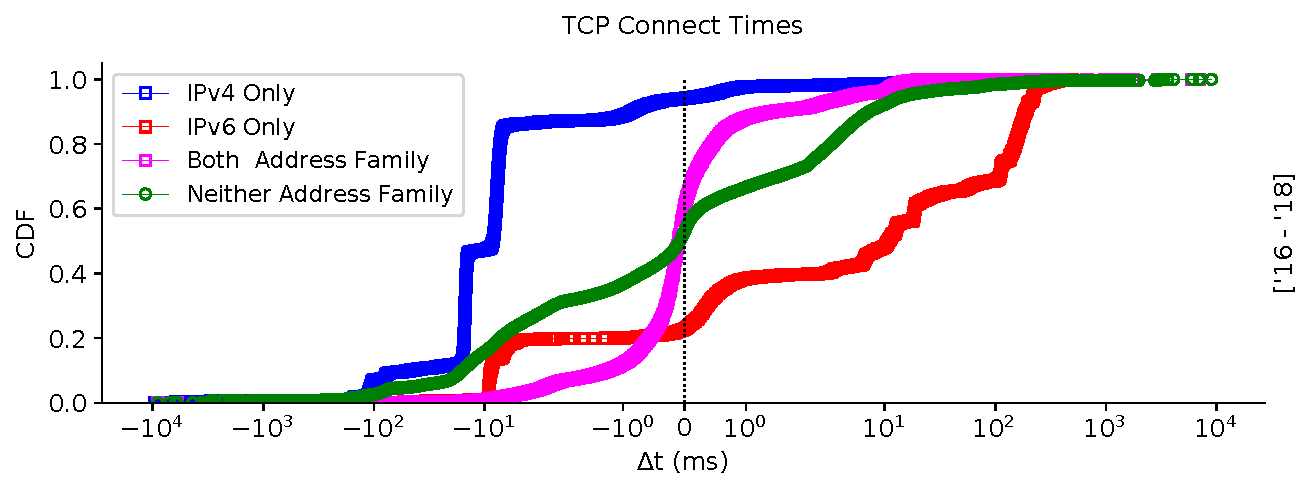
\includegraphics[keepaspectratio, height=5cm, width=8.5cm]{figures/traceroute/netflix-traceroute-median-tcp-cache-pair-cdf.pdf}
	\end{minipage}
	\begin{minipage}{0.5\textwidth}
		\centering
		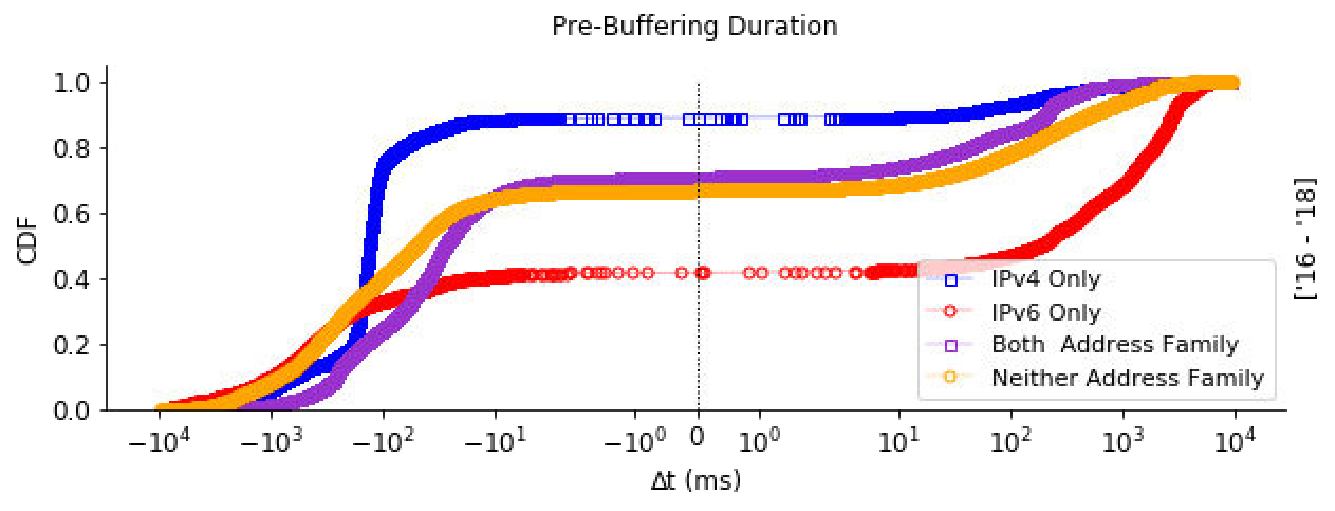
\includegraphics[keepaspectratio, height=5cm, width=8.5cm]{figures/traceroute/netflix-traceroute-median-pd-cache-pair-cdf.pdf}
	\end{minipage}
	\caption[TTL, TCP and Pre-buffering Duration Cache Pair CDF]{CDF over the TTL, TCP and Pre-Buffering duration deltas of destination pairs, identified as cache hits as: 1. IPv4 only, 2. IPv6 Only, 3. Both versions, and 4. Neither Versions. Hitting an ISP cache seems to have improvement over TTL, TCP and Prebuffering Durations.}
	\label{fig:TTL, TCP, and Pre-Buffering Duration Cache Pair CDF}
\end{figure}

Now lets us discuss the plots in \cref{fig:TTL, TCP, and Pre-Buffering Duration Cache Pair CDF}. 

\begin{enumerate}
	\item Here, we can see that the for the IPv4 only case, the curve is shifted towards the left side. For IPv4. TTL measurements of around 47\% are shorter by exactly 4 hops. 
	For TCP connect times around 94\% of the measurements are less than 0 ms and for Pre-buffering duration around 89\% of the measurements are less than 0ms.
	\item For IPv6 only case, the right shift on the curves suggest that the IPv6 caches were hit, and mainly all measurements to the IPv6 cache shows shorter path length. Around 23\% of the measurements for TCP connect times are less than 0 ms,
    and around 42\% of the measurements are less than 0ms for Prebuffering duration.
	\item For both caches i.e. IPv4 and IPv6 requires the same amount of hops, i.e. around 50\% of the measurements are resulting in delta of 0. Concerning the TCP connect times,
    around 60\% of the measurements reached IPv4 faster, and rest 40\% reasched IPv6 faster. In case of Prebuffering durations, around 71\% of the measurements reached IPv4 faster, while the rest 29\% reached IPv6 faster.
    \item For the case where neither cache was hit, i.e. no match between source AS number and Destination AS number, the curve resembles a flat curve.
\end{enumerate}
 
\subsection*{Performance Improvements by Caches}

\begin{figure}[!ht]
	\centering
	\begin{minipage}{0.5\textwidth}
		\centering
		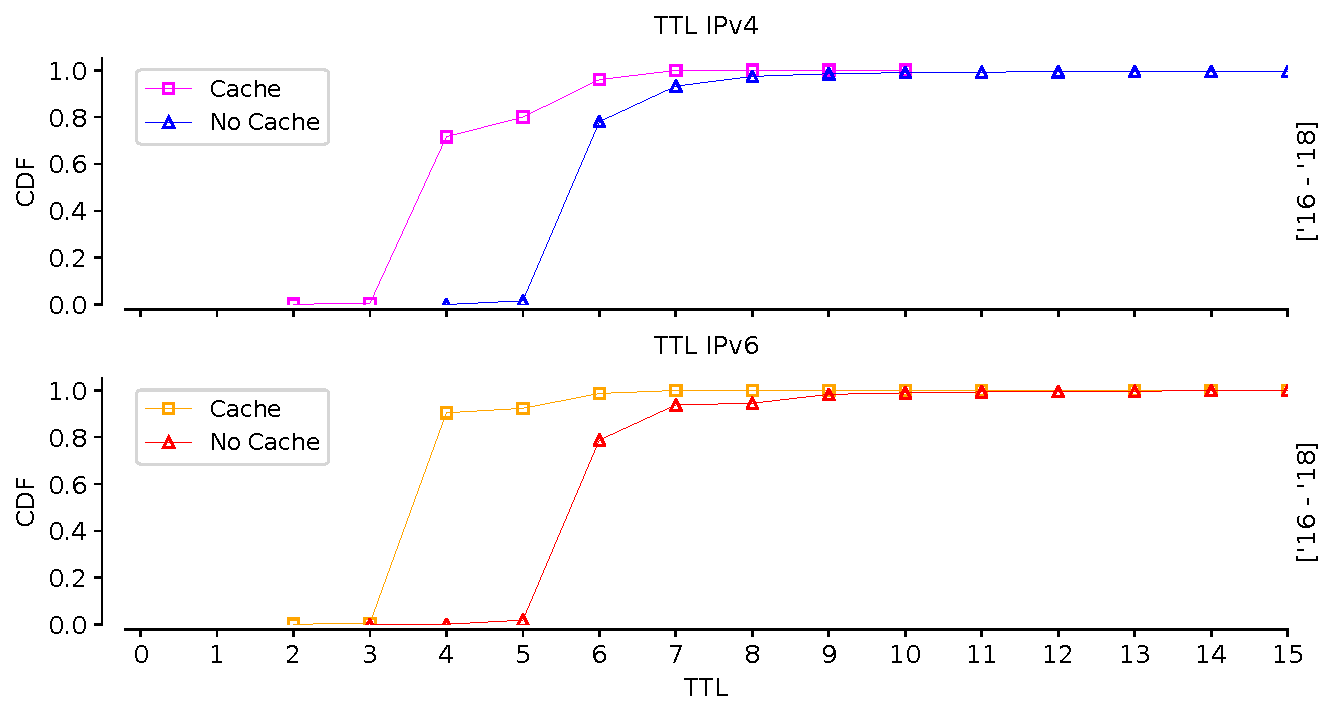
\includegraphics[keepaspectratio, height=5cm, width=8.5cm]{figures/traceroute/netflix-traceroute-cache-vs-origin-cdf.pdf}
	\end{minipage}
	\begin{minipage}{0.5\textwidth}
		\centering
		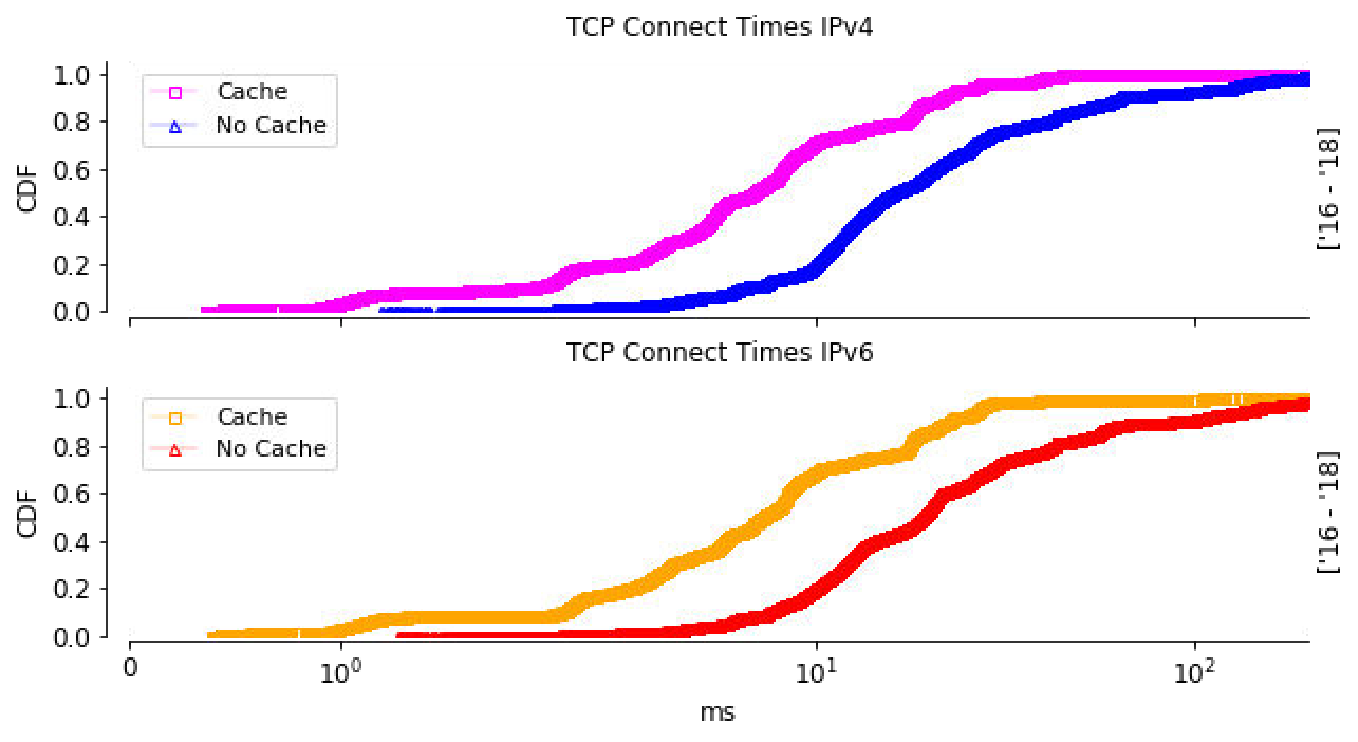
\includegraphics[keepaspectratio, height=5cm, width=8.5cm]{figures/traceroute/netflix-traceroute-tcp-cache-vs-origin-cdf.pdf}
	\end{minipage}
	\begin{minipage}{0.5\textwidth}
		\centering
		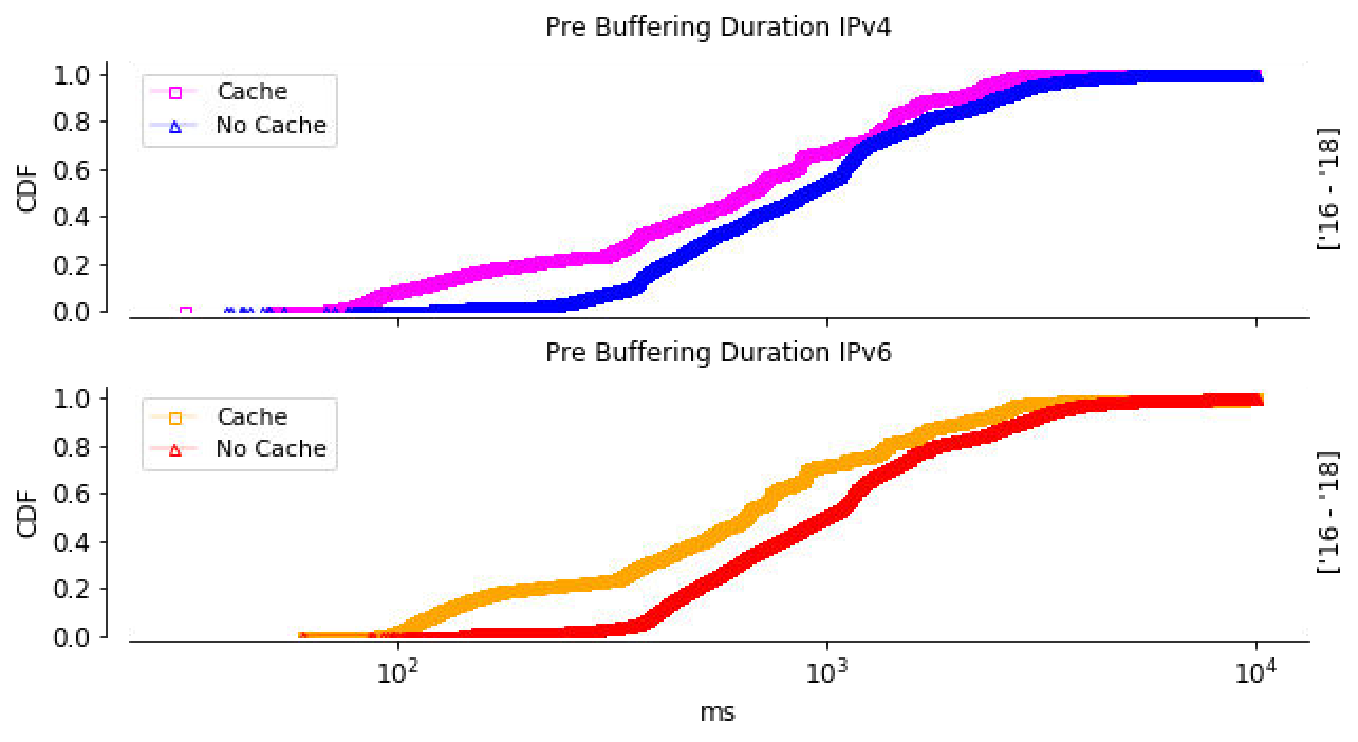
\includegraphics[keepaspectratio, height=5cm, width=8.5cm]{figures/traceroute/netflix-traceroute-pd-cache-vs-origin-cdf.pdf}
	\end{minipage}
	\caption[TTL, TCP and Pre-buffering Duration Cache Vs Origin CDF Absolute]{CDF over the TTL, TCP and Pre-Buffering duration over IPv4 and IPv6. Cache hits curves are above the curves for cache misses, which
	depicts effectiveness of caches with reduced path length (TTL) and latency.}
	\label{fig:TTL, TCP, and PreBuffering Duration Cache Vs Origin CDF Absolute}
\end{figure}

After checking the cache hits, we would like to see the performance impact of these caches. As can be seen from the previous section, a cache hit leads to shorter TTL, 
connect times and pre-buffering duration for that IP address family. Now, to study the impact of this on the performance, we plotted the absolute values of TTL, 
TCP connect times and pre-buffering duration. We considered two cases here, first when the cache was hit and the second when it was missed. 
The criteria of selecting the cache is same as previous, that is, source IP ASN is equal to destination IP ASN.

For \textbf{IPv4}, 96\% of the traces had a TTL of 6, whenever a cache was hit, whereas only 78\% of the cache misses met a TTL of 6. Coming to TCP connect times, cache hit had a connect time of
21 ms for 90\% of the measurements, while for cache misses this is 62 ms. Similarly, for pre-buffering duration, 90\% of the measurements took 1801 ms whenever there was a cache hit, whereas for cache misses
the pre-buffering duration was around 2428 ms.


For \textbf{IPv6}, 99\% of the traces had a TTL of 6, whenever a cache was hit, whereas only 79\% of the cache misses met a TTL of 6. For TCP connect times, cache hit had a connect time of
21 ms, whereas for cache misses this is 69 ms for same number of measurements. Similarly, for pre-buffering durations, 90\% of the measurements took 1992 ms whenever there was cache hit, whereas for cache misses this is 2752 ms
for same number of measurements. 

\FloatBarrier

\section{Path Analysis}

Till now, we were considering only the last rows of the traceroute measurements for a particular measurement. An interesting aspect will be to look into the intermediate 
hops along the path. This could reveal some additional information regarding the state of IPv6 or ISP content caches. We therefore, will consider the 
original \textit{traceroute-filtered} table, with "COMPLETED" results but will contain the total path information for a specific source and destination pair.

\subsection*{Classification of Ases}

We split the data based on the AS type of the intermediate hops i.e. the endpoints. We mapped the \cref{table:endpoint} to the \cref{table:astypes}, 
so that every endpoint belongs to one of the three AS types defined by CAIDA \cite{caida}. These three types are: \textit{Content, Enterprise, or Transit/Access}.

For filtering we followed the same strategy as Viet \cite{viet} did in his study. As per Viet study, we also observed that Content and Enterprise ASes 
were traversed on the first hop, which shouldn't be the case given that first hop is generally the local network router. One possible reason for this could be 
that we were considering non-residential probes as well. Therefore, We further limit the observation to residential probes only. We used the metadata to get the 
probes to filter the probes which are located in a residential setting \cite{metadata}.

\begin{figure}[!ht]
	\centering
	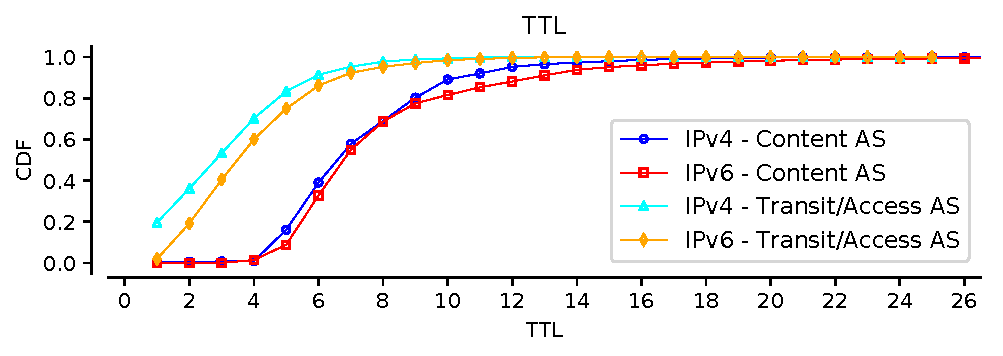
\includegraphics[keepaspectratio, height=5cm, width=15cm]{figures/traceroute/netflix-ttl-by-as-types-cdf.pdf}
	\caption[TTL by AS Types]{CDFs over the TTL values, based on AS type. Both IPv4 and IPv6 showed similar results. TTL value of 5 marks the highest difference between the AS types, indicating that most of the endpoints outside this range belong to Content ASes, and within this range belong to Transit ASes.}
	\label{fig:TTL by AS Types}
\end{figure}

We ignored the "Enterprise" measurements as they were very less compared to Content or Transit type. We could only see 40 "Enterprise" 
labels and thus didn't consider them in our analysis. We can see the distribution of TTL values based on AS types: \textit{Content and Transit}. 
As per the graph, we can see that TTL value of 5 marks the highest difference between the AS types, indicating that most of the endpoints outside this 
range belong to Content ASes, and within this range belong to Transit ASes. Around 83.3\% of the endpoints assigned to Transit/Access ASes had a TTL value of 
less than or equal to 5 for IPv4, and 74.9\% for IPv6. Similarly, around 83.9\% of the IPv4 endpoints classified as Content ASes had TTL values of 5 or greater than 5, 
for IPv6 this percentage was around 91.2\%. 

This shows that TTL value of 5 can be treated as a kind of separator between Transit/Access and Content ASes. Therefore, it signifies that, a Netflix traceroute 
measurement is likely to be an ISP cache if it ends in less than 5 hops. Also, the majority of ASes within the range of 5 were seen to be located in Internet Service 
Provider networks. Similarly, TTL value of 5 and above suggests that the AS is most likely a Content AS.